%% ma: L12-B01-0042
%% lop: 12
%% chuong: 1
%% bai: 1
%% dang: 12.1.26
%% loai: TN4
%% muc: TH
%% dap_an: "C"
%% nguon: "Ảnh giáo viên gửi 05/11/2026 (M11): Kiểm tra giữa HK1 Toán 12 (2026-2027), THPT Hồ Thị Bi (TP.HCM), mã đề 1133, Phần I Câu 16"
%% kien_thuc: "Bài 1 (cực trị của hàm số đọc từ bảng biến thiên, hàm số không xác định tại một điểm)"
%% trang_thai: chinh-thuc
%% ghi_chu: "Giáo viên đã duyệt 05/11/2026 (cả dạng mới). Đề gốc không kèm đáp án; đã giải độc lập."
\begin{ex}
Cho hàm số $y=g(x)$ xác định với mọi $x\ne4$ và có bảng biến thiên như sau:
\begin{center}
\begin{tikzpicture}
  \tkzTabInit[lgt=1.5,espcl=2]{$x$/.8,$g'(x)$/.8,$g(x)$/2.4}{$-\infty$,$1$,$4$,$6$,$+\infty$}
  \tkzTabLine{,+,0,-,d,-,0,+,}
  \tkzTabVar{-/$-\infty$,+/$-3$,-D+/$-\infty$/$+\infty$,-/$1$,+/$+\infty$}
\end{tikzpicture}
\end{center}
Giá trị cực tiểu của hàm số đã cho bằng
\choice{$6$}{$4$}{\True $1$}{$-3$}
\loigiai{$g'(x)$ đổi dấu từ âm sang dương khi qua $x=6$ nên hàm số đạt cực tiểu tại $x=6$, giá trị cực tiểu là $g(6)=1$.
Hàm số không xác định tại $x=4$ nên $x=4$ không phải điểm cực trị. $-3$ là giá trị cực đại tại $x=1$.}
\end{ex}
